\documentclass{beamer}
\usepackage{natbib}
\bibliographystyle{apalike}

\author{Ignas Ramanauskas}

\begin{document}

\begin{frame}
  \frametitle{GC Base Counts and Their Effects On Genomes}
  \footnotesize{Ignas Ramanauskas}
  \normalsize
  2023
\end{frame}

\begin{frame}
  \frametitle{Introduction}
  Using different techniques in Bash scripting and with the help of Vinogradov's published paper we analyzed GC content in yeast genomes to understand how their genetic makeup affects their functionality, mainly thermostability and bendability.
\end{frame}

\begin{frame}
  \frametitle{Methods}
  \begin{itemize}
      \item Using multiple scripts like fasta-unfold, find-orfs and gc-count, aswell as python script, were used to analyze and modify data from genome fasta files and provide images with useful data.
      \item In A. E. Vinogradov's paper the genome data was collected from GeneBank. Bendability and curvature of nucleotide sequences were determined using the trinucleotide table of consensus values obtained from DNase I digestion and nucleosome positioning studies. The thermostability was determined using a unified dinucleotide table for free energy of melting [\cite{Vinogradov2003}].
  \end{itemize}
  
\end{frame}

\begin{frame}
  \frametitle{Results}
  \begin{itemize}
      \item According to A. E. Vinogradov's research paper, it was found that higher GC percentages correlated with a slight decrease of thermostability
      \item With increased elevation of GC percentages it was seen that bendability also increased
      
  \end{itemize}
\end{frame}

\begin{frame}
  \frametitle{Results}
    In Figure 1, the average percentages of GC bases in CLIB215 yeast species are presented. The GC content is consistently around 38 percent.
  \begin{figure}
    \centering
    \begin{minipage}{0.48\textwidth}
      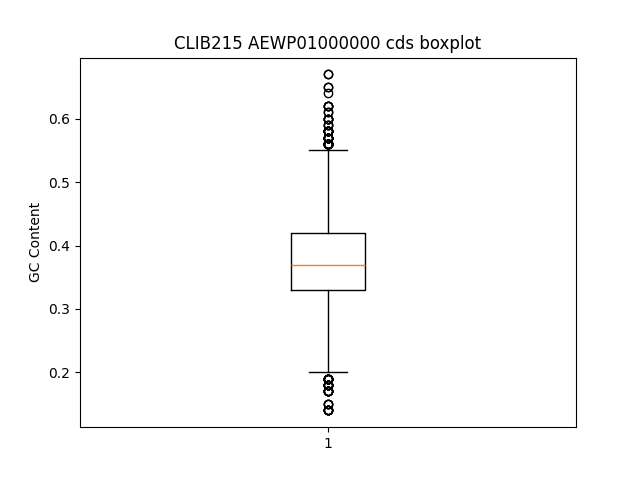
\includegraphics[width=\linewidth]{images/CLIB215_AEWP01000000_cds_boxplot.png}
    \end{minipage}\hfill
    \begin{minipage}{0.48\textwidth}
      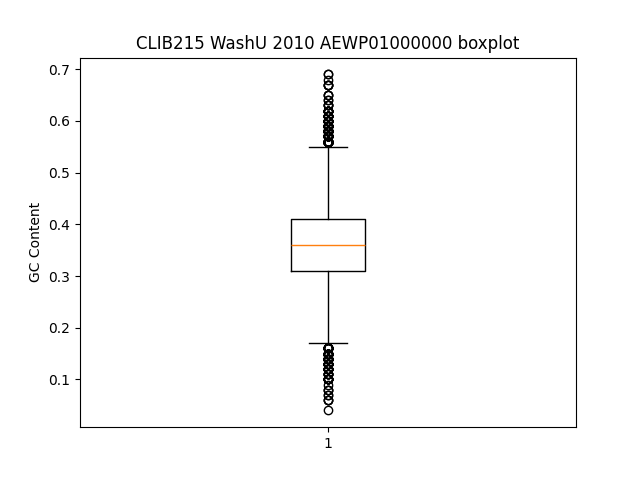
\includegraphics[width=\linewidth]{images/CLIB215_WashU_2010_AEWP01000000_boxplot.png}
    \end{minipage}
    \caption{Average GC content percentages in CLIB215 yeast species from different databases.}
  \end{figure}
\end{frame}

\begin{frame}
  \frametitle{Results}
    In this image we can see percentages of EC9-8 yeast species. This image provides us with a similar result as the first one.
  \begin{figure}
    \centering
    \begin{minipage}{0.48\textwidth}
      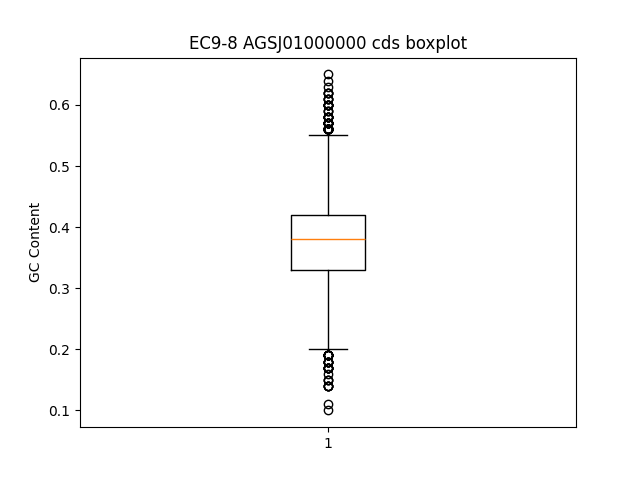
\includegraphics[width=\linewidth]{images/EC9-8_AGSJ01000000_cds_boxplot.png}
    \end{minipage}\hfill
    \begin{minipage}{0.48\textwidth}
      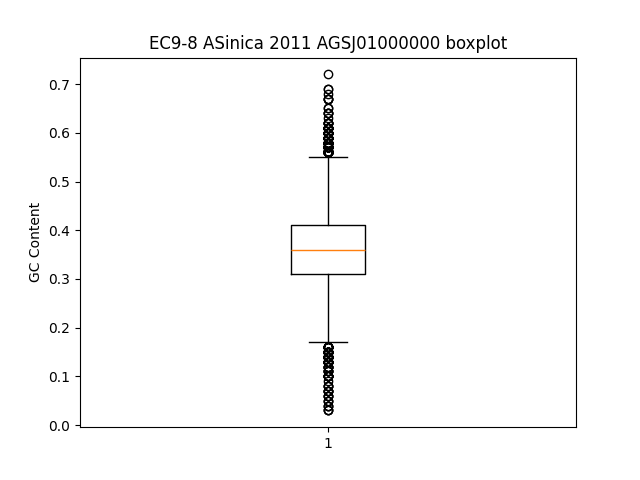
\includegraphics[width=\linewidth]{images/EC9-8_ASinica_2011_AGSJ01000000_boxplot.png}
    \end{minipage}
    \caption{Average GC content percentages in EC9-8 yeast species from different databases.}
  \end{figure}
\end{frame}

\begin{frame}
  \frametitle{Conclusions}
  \begin{itemize}
      \item To summarise our results, according to A. E. Vinogradov, we saw that increased GC percentages in genomes resulted in slightly less thermostability, but with increased DNA's bendability, which could hint us that places with higher GC percentages are more likely to be coding regions.
      \item When comparing GC counts in different yeast species, we saw a similarity of GC percentages across all yeast species, which was expected. The differences in outliers between same species of yeast could be explained by having data from different databases.
  \end{itemize}
  
\end{frame}

\begin{frame}
\frametitle{References}
  \bibliography{reports/source}
\end{frame}


  

\end{document}

